\documentclass[a4paper]{article}
\usepackage{booktabs}
\usepackage{geometry}
\geometry{
  top=1in,
  inner=1in,
  outer=1in,
  bottom=1in,
  headheight=3ex,
  headsep=2ex
}
\usepackage{amssymb,amsmath}
\usepackage{fontspec}
\usepackage[CJKbookmarks, colorlinks, bookmarksnumbered=true,pdfstartview=FitH,linkcolor=black,citecolor=black]{hyperref}
\usepackage{xeCJK}
\usepackage{xltxtra,xunicode}
\usepackage{listings}
\usepackage{xcolor}
\usepackage{array}
\usepackage{float}

\lstset{basicstyle=\footnotesize\ttfamily,        % size of fonts used for the code
        columns=fullflexible,
        numbers=left,
        numberstyle=\tiny,
        keywordstyle=\color{blue},
        stringstyle=\color[rgb]{0,0.6,0},
        commentstyle=\color[cmyk]{1,0,1,0},
        frame=shadowbox,
        escapeinside=``,
        breaklines=true,
        extendedchars=false,
        xleftmargin=2em,xrightmargin=2em, aboveskip=1em,
        tabsize=4, %tab size
        showspaces=false %no space
       }

\newcommand{\tightlist}{
  \setlength{\itemsep}{0pt}\setlength{\parskip}{0pt}}

% font
\setCJKmainfont[AutoFakeBold]{文泉驿微米黑}
\setmainfont[AutoFakeBold]{Segoe UI}
\setromanfont[AutoFakeBold]{Segoe UI}
\setmonofont[Mapping={}]{Monaco}
\linespread{1.2}\selectfont
\XeTeXlinebreaklocale "zh" 
\setcounter{secnumdepth}{3}
\begin{document}
\title{\Huge Java技术\\ 第二次上机报告}
\author { \vspace{12cm} \\ \LARGE 班级:  1413014  \\ \LARGE 姓名:  乔新文   \\ \LARGE 学号:14130140393} 
\date{ \vspace{4cm} 2017.4.13}

\maketitle
\clearpage

\tableofcontents

\clearpage

\section{综述}

本文档将阐述《Java技术》第二次上机代码的详细设计及实现。\\

为节约篇幅,文档中对上机要求中已有的部分将不再复述,仅对总体的设计思路,要求外添加的内容和部分重要的代码做出说明。\\

本次上机实验所用代码均为UTF-8编码,编译过程中如果报错请在编译命令中加上“-encoding UTF-8”选项。\\

本次上机所有代码均在本机(Win10 10586 64位)上经过测试并运行正常,其他环境下则未经测试。

\section{题目一}

\subsection{题目}

Command Oriented Personal Information Manager

\subsection{设计阐述}

PIM系统类关系图:\\
\begin{figure}[h]
    \centering
    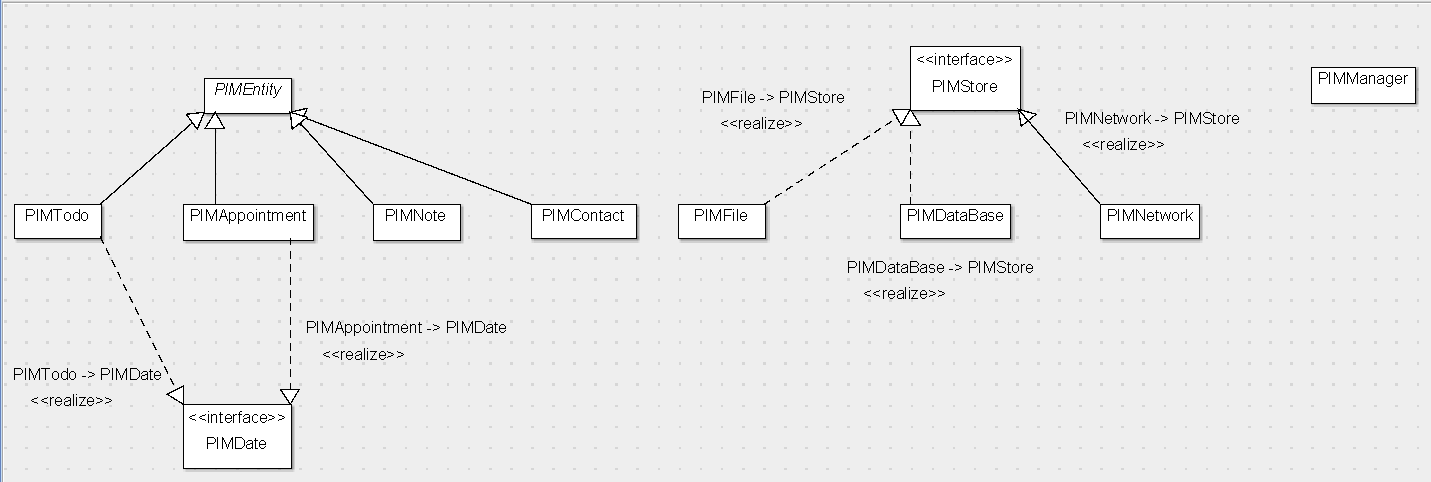
\includegraphics[width=16cm]{classall.png}\\
\end{figure}

    \subsubsection{PINDate接口}
    接口中声明了三个对日期的操作,分别为:读取日期,设置日期以及格式化输出日期。
        \begin{figure}[h]
            \centering
            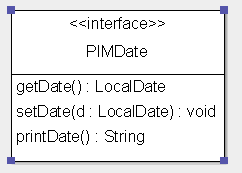
\includegraphics[width=4cm]{date.png}
        \end{figure}\\
        

    \subsubsection{PIMTodo,\ PIMNote,\ PIMContact,\ PINTodo}
        四个类都继承子 \ PIMEntity\ 父类,且均额外添加了一个静态方法 \ FromString(s:String) \  用来与重写的\ toString()\ 方法配合实现基于字符串的序列化和反序列化。\\
        其中PINTodo,PINTodo继承并实现了PIMDate接口。
        \begin{figure}[h]
            \centering
            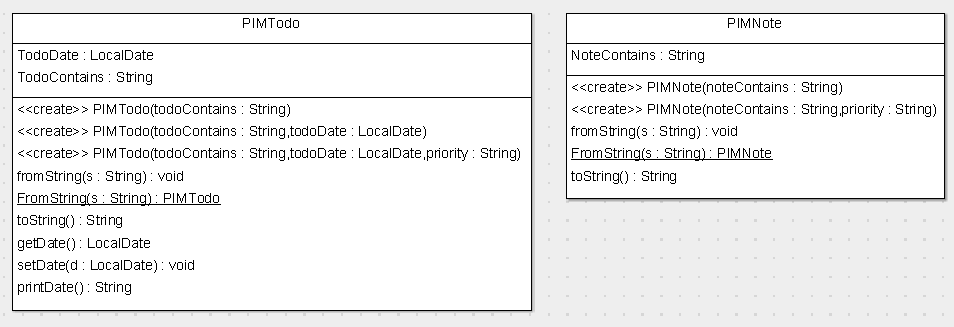
\includegraphics[width=18cm]{tandn.png}\\
            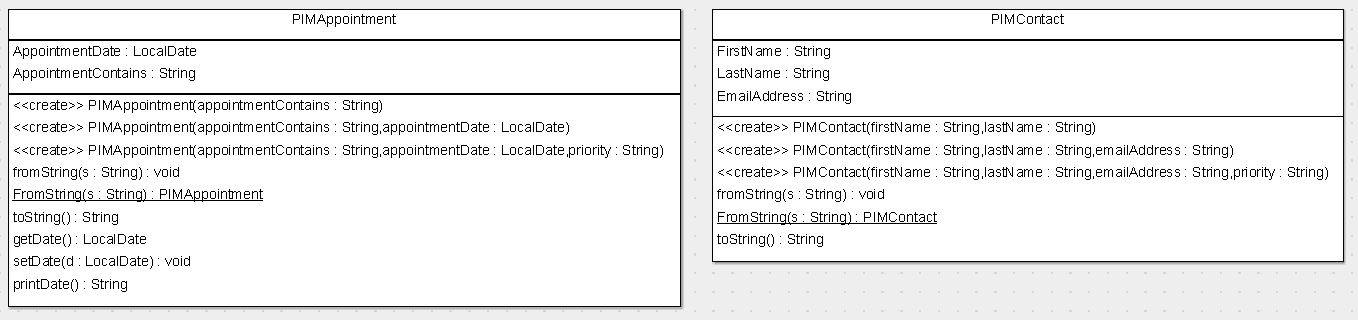
\includegraphics[width=18cm]{aandc.png}
        \end{figure}\\

    \subsubsection{PIMStore}
        设计这个接口为的是尽可能在一定程度上屏蔽访问文件,数据库,网路时的差异,借鉴了Unix中“everything is a file”的设计思想,将访问文件,数据库,网络的操作抽象为\ Open(),Read(),Write(),Close()\ 四个方法。\\
        在PIM系统中,任何对文件,数据库,网络的操作都必须遵循先Open,再Read或Write,最后Close的过程,并且在一次操作中限制不允许同时Read和Write以保证数据的一致性。
        \begin{figure}[h]
            \centering
            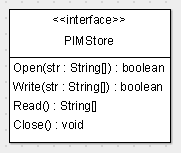
\includegraphics[width=4cm]{store.png}
        \end{figure}\\

    \subsubsection{PIMManager}
        PIMManager最为整个PIM系统的master unit,接受命令行传入的参数初始化整个系统并通过Run()进入一级指令解析器,按照命令解析结果调用相应功能。
        \begin{figure}[h]
            \centering
            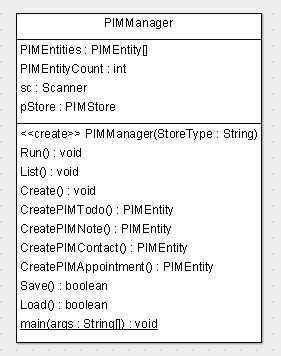
\includegraphics[width=5cm]{mamager.png}
        \end{figure}\\
\subsection{代码片段}

提示用户输入日期并解析为LocalDate对象实例。

\begin{lstlisting}[language=Java]
    System.out.println("Enter date for todo item:(like 04/20/2017):");
    LocalDate TodoDate = null;
    String DateString = sc.nextLine();
    try{
        TodoDate = LocalDate.parse(DateString,DateTimeFormatter.ofPattern("MM/dd/yyyy"));
    }
    catch(DateTimeParseException e){
        System.out.println("Date Format Error, Go Back Create Item.");
        return null;
    }
\end{lstlisting}

PIMTodo中实现的格式化输出日期字符串

\begin{lstlisting}[language=Java]
    public String printDate(){
        return TodoDate.format(DateTimeFormatter.ofPattern("yyyy-MM-dd"));
    }
\end{lstlisting}

PIMTodo中实现的toString()

\begin{lstlisting}[language=Java]
    public String toString(){
        return "Type: PIMTodo    " + "Priority: " + getPriority() + "    Date: " + printDate() + "    " + TodoContains;
    }
\end{lstlisting}

PIMTodo中实现的实例fromString()

\begin{lstlisting}[language=Java]
    public void fromString(String s)
    {
        //s likes "Type: PIMTodo    Priority: normal    Date: 2017-04-20    text""
        String[] ss = s.split("(Type: )|(Priority: )|(Date: )|(    )");
        String[] sss = new String[4];
        int temp = 0;
        for (String var : ss) {
            if(temp >= 4){
                System.out.println("Input String can't to PIMTodo.");
                return;
            }
            if(!var.equals("")){
                sss[temp] = var;
                temp ++;
            }
        }
        if(!sss[0].equals("PIMTodo")){
            System.out.println("Input String can't to PIMTodo.");
            return;
        }
        setPriority(sss[1]);
        TodoDate = LocalDate.parse(sss[2],DateTimeFormatter.ofPattern("yyyy-MM-dd"));
        TodoContains = sss[3];
    }
\end{lstlisting}

PIMTodo中实现的静态FromString()

\begin{lstlisting}[language=Java]
    public static PIMTodo FromString(String s)
    {
        //s likes "Type: PIMTodo    Priority: normal    Date: 2017-04-20    text""
        String[] ss = s.split("(Type: )|(Priority: )|(Date: )|(    )");
        String[] sss = new String[4];
        int temp = 0;
        for (String var : ss) {
            if(temp >= 4){
                System.out.println("Input String can't to PIMTodo.");
                return null;
            }
            if(!var.equals("")){
                sss[temp] = var;
                temp ++;
            }
        }
        if(!sss[0].equals("PIMTodo")){
            System.out.println("Input String can't to PIMTodo.");
            return null;
        }

        return new PIMTodo(sss[3], LocalDate.parse(sss[2],DateTimeFormatter.ofPattern("yyyy-MM-dd")), sss[1]);
    }
\end{lstlisting}


PIMFile中实现的Open()操作

\begin{lstlisting}[language=Java]
    public boolean Open(String[] str){
        try{
            file = new File(str[0]);
            if(file.exists()&&file.isFile()){
                //file.delete();
            }
            else{
                file.createNewFile();
            }
            return true;
        }
        catch(Exception e){
            System.out.println("Open File failed!.");
            file = null;
            return false;
        }
    }
\end{lstlisting}

PIMFile中实现的Read()操作

\begin{lstlisting}[language=Java]
    public String[] Read(){
        if(file == null){
            System.out.println("Read File failed!.");
            return null;
        }
        try{
            ArrayList<String> tempList = new ArrayList<String>();
            String temp = null;
            BufferedReader br = new BufferedReader(new FileReader(file));
            while((temp = br.readLine()) != null){
                tempList.add(temp);
            }
            br.close();
            return tempList.toArray(new String[tempList.size()]);
        }
        catch(Exception e){
            System.out.println("Read File failed!.");
            return null;
        }
    }
\end{lstlisting}

PIMFile中实现的Write()操作

\begin{lstlisting}[language=Java]
    public boolean Write(String[] str){
        if(file == null){
            System.out.println("Write File failed!.");
            return false;
        }
        try{
            BufferedWriter bw = new BufferedWriter(new FileWriter(file));
            for (String var : str) {
                bw.write(var);
                bw.newLine();
            }
            bw.flush();
            bw.close();
            return true;
        }
        catch(Exception e){
            System.out.println("Write File failed!.");
            return false;
        }

    }
\end{lstlisting}

PIMManager中Run()的一级命令解析器

\begin{lstlisting}[language=Java]
    public void Run(){
        System.out.println("Welcome to PIM.");
        String command = "";
        while(true){
            System.out.println("---Enter a command (suported commands are List Create Save Load Quit)---");
            command = sc.nextLine();
            switch(command.toLowerCase()){
                case "list":{
                    List();
                    break;
                }
                case "create":{
                    Create();
                    break;
                }
                case "save":{
                    Save();
                    break;
                }
                case "load":{
                    Load();
                    break;
                }
                case "quit":{
                    return;
                }
                default:{
                    System.out.println("Command Not Find.");
                }
            }
        }
    }
\end{lstlisting}

PIMManager中实现的List(),Save(),Load()操作

\begin{lstlisting}[language=Java]
    public void List(){
        System.out.printf("There are %d items.\n",PIMEntityCount);
        for(int i = 0; i < PIMEntityCount; i++){
            System.out.printf("Item %d:", i);
            System.out.println(PIMEntities[i].toString());
        }
    }
    public boolean Save(){
        String[] PIMEntitiesInfo =  new String[PIMEntityCount];
        String[] FileNameAndPath = new String[1];

        System.out.print("Enter The File Name With Path:");
        FileNameAndPath[0] = sc.nextLine();

        for(int i = 0; i < PIMEntityCount; i++){
            PIMEntitiesInfo[i] = PIMEntities[i].toString();
        }

        if(pStore.Open(FileNameAndPath) && pStore.Write(PIMEntitiesInfo)){
            pStore.Close();
            System.out.println("Save Succeed!.");
            return true;
        }
        else{
            pStore.Close();
            return false;
        }
    }
    public boolean Load(){
        String[] FileNameAndPath = new String[1];
        System.out.print("Enter The File Name With Path:");
        FileNameAndPath[0] = sc.nextLine();
        if(!pStore.Open(FileNameAndPath)){
            return false;
        }
        String[] PIMEntitiesInfo = pStore.Read();
        if(PIMEntitiesInfo == null){
            pStore.Close();
            return false;
        }
        PIMEntityCount = 0;
        for(int i = 0; i<PIMEntitiesInfo.length;i++){
            try{
                switch(PIMEntitiesInfo[i].substring(0, 13)){
                    case "Type: PIMTodo":{
                        PIMEntities[PIMEntityCount] = PIMTodo.FromString(PIMEntitiesInfo[i]);
                        PIMEntityCount++;
                        break;
                    }
                    case "Type: PIMNote":{
                        PIMEntities[PIMEntityCount] = PIMNote.FromString(PIMEntitiesInfo[i]);
                        PIMEntityCount++;
                        break;
                    }
                    case "Type: PIMAppo":{
                        PIMEntities[PIMEntityCount] = PIMAppointment.FromString(PIMEntitiesInfo[i]);
                        PIMEntityCount++;
                        break;
                    }
                    case "Type: PIMCont":{
                        PIMEntities[PIMEntityCount] = PIMContact.FromString(PIMEntitiesInfo[i]);
                        PIMEntityCount++;
                        break;
                    }
                    default:{
                        System.out.println(PIMEntitiesInfo[i] + " Can't Parse");
                    }
                }
            }
            catch(IndexOutOfBoundsException e){
                System.out.println(PIMEntitiesInfo[i] + " Can't Parse");
                continue;
            }
        }
        pStore.Close();
        System.out.println("Load Succeed!.");
        return true;
    }
\end{lstlisting}

PIMManager中实现的CreatePIMTodo()操作

\begin{lstlisting}[language=Java]
    private PIMEntity CreatePIMTodo(){
        System.out.println("Enter date for todo item:(like 04/20/2017):");
        LocalDate TodoDate = null;
        String DateString = sc.nextLine();
        try{
            TodoDate = LocalDate.parse(DateString,DateTimeFormatter.ofPattern("MM/dd/yyyy"));
        }
        catch(DateTimeParseException e){
            System.out.println("Date Format Error, Go Back Create Item.");
            return null;
        }

        System.out.println("Enter date for todo text:");
        String TextString = sc.nextLine();

        System.out.println("Enter date for todo priority:");
        String PriorityString = sc.nextLine();

        return new PIMTodo(TextString, TodoDate, PriorityString);
    }
\end{lstlisting}

最后则是PIM系统的启动代码

\begin{lstlisting}[language=Java]
    public static void main(String[] args) {
        PIMManager m = null;
        if(args.length == 0){
            m = new PIMManager(null);
        }
        else{
            m = new PIMManager(args[0]);
        }
        
        m.Run();
    }
\end{lstlisting}

\subsection{测试}
\begin{lstlisting}[language=Java,numbers=none]
---Enter a command (suported commands are List Create Save Load Quit)---
list
There are 0 items.
---Enter a command (suported commands are List Create Save Load Quit)---
load
Enter The File Name With Path:save
Load Succeed!.
---Enter a command (suported commands are List Create Save Load Quit)---
list
There are 2 items.
Item 0:Type: PIMTodo    Priority: normal    Date: 2017-04-13    Learn Java
Item 1:Type: PIMNote    Priority: normal    deal with java homework
---Enter a command (suported commands are List Create Save Load Quit)---
create note
Command Not Find.
---Enter a command (suported commands are List Create Save Load Quit)---
create
Enter an item type ( todo, note, contact or appointment ) or quit to exit create item
note
Enter date for note text:
play game
Enter date for note priority:
normal
Create Item Succeed!
---Enter a command (suported commands are List Create Save Load Quit)---
list
There are 3 items.
Item 0:Type: PIMTodo    Priority: normal    Date: 2017-04-13    Learn Java
Item 1:Type: PIMNote    Priority: normal    deal with java homework
Item 2:Type: PIMNote    Priority: normal    play game
---Enter a command (suported commands are List Create Save Load Quit)---
load
Enter The File Name With Path:savefile
Load Succeed!.
---Enter a command (suported commands are List Create Save Load Quit)---
\end{lstlisting}

\section{题目二}

\subsection{题目}

Class Substring

\subsection{设计阐述}
Java中String实例的substring()方法j接受的参数是截取部分的起始下标beginindex和结束下标endindex,可以计算出:\[beginindex=index,\] \[endindex=index+length\]
其中可能引发的异常为获取参数字符串时的\emph{ArrayIndexOutOfBoundsException}异常,\emph{Integer.parseInt()}方法解析字符串时的\emph{NumberFormatException}异常以及\emph{String}类型的\emph{substring}方法抛出的\emph{IndexOutOfBoundsException}异常,\\
由于设计时将该方法设计的向库方法靠拢,故此处不再打印错误信息提示用户而是将异常捕获后再次抛出,由上层调用者进行处理。
\subsection{实现代码}

\begin{lstlisting}[language=Java]
import java.lang.*;
public class  Substring {
    public static void main(String[] args) {
        try{
            String str = args[0].substring(Integer.parseInt(args[1]), Integer.parseInt(args[1]) + Integer.parseInt(args[2]));
            System.out.println(str);
        }
        catch(ArrayIndexOutOfBoundsException e){
            throw new IllegalArgumentException();
        }
        catch(NumberFormatException e){
            throw e;
        }
        catch(IndexOutOfBoundsException e){
            throw new IllegalArgumentException();
        }
        catch(Exception e){
            throw e;
        }
    }
}
\end{lstlisting}

\subsection{测试}

\begin{lstlisting}[language=Java,numbers=none]
PS G:\Java\JavaHomework\HW2> java Substring Jello 1 3
ell
PS G:\Java\JavaHomework\HW2> java Substring "Hello World" 0 5
Hello
PS G:\Java\JavaHomework\HW2> java Substring OneTwoThree 5 1
o
PS G:\Java\JavaHomework\HW2> java Substring OneTwoThree 5 15
Exception in thread "main" java.lang.IllegalArgumentException
        at Substring.main(Substring.java:21)
\end{lstlisting}

\section{题目三}
\subsection{题目}
Calendar generating program
\subsection{设计阐述}
欲输出某月的日历,需要的关键数据为本月一日的星期数和本月的天数。\\

\subsection{代码片段}
获取当前月份的第一天

\begin{lstlisting}[language=Java]
    LocalDate ldb = null;
    try{
        if(args[0].length() == 1){
            args[0] = "0" + args[0];
        }
        ldb = LocalDate.parse(args[0] + args[1] + "01",DateTimeFormatter.ofPattern("MMyyyydd"));
    }
    catch(Exception e){
        ldb = LocalDate.now().with(TemporalAdjusters.firstDayOfMonth());
    }
\end{lstlisting}

获取当前月份的最后一天

\begin{lstlisting}[language=Java]
    LocalDate lde = ldb.with(TemporalAdjusters.lastDayOfMonth())
\end{lstlisting}

打印日历的第一、二行

\begin{lstlisting}[language=Java]
    String mouth = ldb.getMonth().toString();
    System.out.println(mouth.substring(0, 1) + mouth.substring(1).toLowerCase() + " " + Integer.toString(ldb.getYear()));
    System.out.println("Su Mo Tu We Th Fr Sa");
\end{lstlisting}

获取当前月份的天数

\begin{lstlisting}[language=Java]
    lde.getDayOfMonth() + ldb.getDayOfWeek().getValue()
\end{lstlisting}

打印日历的每一行并按星期换行

\begin{lstlisting}[language=Java]
    for(int i = 1; i<=lde.getDayOfMonth() + ldb.getDayOfWeek().getValue(); i++){
        if(i<=ldb.getDayOfWeek().getValue()){
            System.out.print("   ");
        }
        else{
            System.out.print(String.format("%02d ", i - ldb.getDayOfWeek().getValue()));
        }
        if(i%7==0){
            System.out.println();
        }
    }
\end{lstlisting}

整体代码

\begin{lstlisting}[language=Java]
import java.time.*;
import java.time.temporal.TemporalAdjusters;
import java.time.format.DateTimeFormatter;
public class cal {
    public static void main(String[] args) {
        LocalDate ldb = null;
        try{
            if(args[0].length() == 1){
                args[0] = "0" + args[0];
            }
            ldb = LocalDate.parse(args[0] + args[1] + "01",DateTimeFormatter.ofPattern("MMyyyydd"));
        }
        catch(Exception e){
            ldb = LocalDate.now().with(TemporalAdjusters.firstDayOfMonth());
        }
        PrintfMouth(ldb);
    }

    public static void PrintfMouth(LocalDate ldb){
        LocalDate lde = ldb.with(TemporalAdjusters.lastDayOfMonth());
        
        String mouth = ldb.getMonth().toString();
        System.out.println(mouth.substring(0, 1) + mouth.substring(1).toLowerCase() + " " + Integer.toString(ldb.getYear()));
        System.out.println("Su Mo Tu We Th Fr Sa");

        for(int i = 1; i<=lde.getDayOfMonth() + ldb.getDayOfWeek().getValue(); i++){
            if(i<=ldb.getDayOfWeek().getValue()){
                System.out.print("   ");
            }
            else{
                System.out.print(String.format("%02d ", i - ldb.getDayOfWeek().getValue()));
            }
            if(i%7==0){
                System.out.println();
            }
        }
    }
}
\end{lstlisting}

\subsection{测试}
\begin{lstlisting}[language=Java,numbers=none]
PS G:\Java\JavaHomework\HW2> java cal 4 2025
April 2025
Su Mo Tu We Th Fr Sa
      01 02 03 04 05
06 07 08 09 10 11 12
13 14 15 16 17 18 19
20 21 22 23 24 25 26
27 28 29 30
PS G:\Java\JavaHomework\HW2> java cal
April 2017
Su Mo Tu We Th Fr Sa
                  01
02 03 04 05 06 07 08
09 10 11 12 13 14 15
16 17 18 19 20 21 22
23 24 25 26 27 28 29
30
\end{lstlisting}
\end{document}